\documentclass[12pt,a4paper]{article}
\usepackage{task}

\newcommand{\contestName}{MateInfoUB}
\newcommand{\contestDates}{18 Mai 2025}
\newcommand{\contestPlace}{Facultatea de Matematic\v a-Informatic\v a}
\newcommand{\contestRound}{Runda Final\v a}
%\newcommand{\contestRound}{Rund\v a de Test}
\newcommand{\statementLanguage}{Rom\^ an\v a (Oficial)}
\newcommand{\taskShortName}{Strigoi}


\definecolor{Brown}{cmyk}{0,0.81,1,0.60}
\definecolor{OliveGreen}{cmyk}{0.64,0,0.95,0.40}
\definecolor{CadetBlue}{cmyk}{0.62,0.57,0.23,0}
\definecolor{lightlightgray}{gray}{0.9}

\lstset{
% language=C++,                             % Code langugage
basicstyle=\ttfamily,                   % Code font, Examples: \footnotesize, \ttfamily
keywordstyle=\bfseries,        % Keywords font ('*' = uppercase)
commentstyle=\color{gray},              % Comments font
columns=flexible,
% numbers=left,                           % Line nums position
% numberstyle=\tiny,                      % Line-numbers fonts
% stepnumber=1,                           % Step between two line-numbers
% numbersep=5pt,                          % How far are line-numbers from code
% backgroundcolor=\color{lightlightgray}, % Choose background color
% frame=none,                             % A frame around the code
% tabsize=2,                              % Default tab size
% captionpos=b,                           % Caption-position = bottom
% breaklines=true,                        % Automatic line breaking?
% breakatwhitespace=false,                % Automatic breaks only at whitespace?
% showspaces=false,                       % Dont make spaces visible
% showtabs=true,                         % Dont make tabls visible
}


\setlength{\parskip}{0pt}

\begin{document}
% Tex fragment for task statement headers
% Usage:
%       % Defining parameters required for header
%       \newcommand{\contestName}{Name of the Contest Series}
%       \newcommand{\contestDates}{Month 1 -- 8 20XX}
%       \newcommand{\contestPlace}{City, Country}
%       \newcommand{\contestRound}{Day 1}
%       \newcommand{\statementLanguage}{en (US)}
%       \newcommand{\taskShortName}{task_short_name}
%       % Tex fragment for task statement headers
% Usage:
%       % Defining parameters required for header
%       \newcommand{\contestName}{Name of the Contest Series}
%       \newcommand{\contestDates}{Month 1 -- 8 20XX}
%       \newcommand{\contestPlace}{City, Country}
%       \newcommand{\contestRound}{Day 1}
%       \newcommand{\statementLanguage}{en (US)}
%       \newcommand{\taskShortName}{task_short_name}
%       % Tex fragment for task statement headers
% Usage:
%       % Defining parameters required for header
%       \newcommand{\contestName}{Name of the Contest Series}
%       \newcommand{\contestDates}{Month 1 -- 8 20XX}
%       \newcommand{\contestPlace}{City, Country}
%       \newcommand{\contestRound}{Day 1}
%       \newcommand{\statementLanguage}{en (US)}
%       \newcommand{\taskShortName}{task_short_name}
%       \input{header.tex}
%


%--------------------- tools ----------------------
\makeatletter
% \expandafter for the case that the parameter is given in a command
\newcommand{\escapeUnderscores}[1]{\expandafter\@repl@underscores#1_\relax}
\def\@repl@underscores#1_#2\relax{%
    \ifx \relax #2\relax
        % #2 is empty => finish
        #1%
    \else
        % #2 is not empty => underscore was contained, needs to be replaced
        #1%
        \textunderscore
        % continue replacing
        % #2 ends with an extra underscore so I don't need to add another one
        \@repl@underscores#2\relax
    \fi
}
\makeatother
% -------------------------------------------------

\vspace*{-3em}\hspace*{-.5cm}
\begin{tabular}{ccl}
    \hspace{1mm}
\includegraphics[width=2.2cm,valign=b]{logo.jpeg}
    & 
    \begin{minipage}[b]{10cm}
        \setlength{\baselineskip}{1.05\baselineskip}
        \sffamily
        \makebox[0pt][l]{\bfseries \large \contestName}  \\
        \contestDates \\ 
        \contestPlace
    \end{minipage}
    & 
    \begin{minipage}[b]{3.7cm}
        \begin{flushright}
            \makebox[0pt][r]{\ttfamily \bfseries \large \escapeUnderscores{\taskShortName}}  \\[.2em]
            \sffamily
            \contestRound \\
            \statementLanguage
        \end{flushright}
    \end{minipage}
\end{tabular} 
\hrule height .06em
%


%--------------------- tools ----------------------
\makeatletter
% \expandafter for the case that the parameter is given in a command
\newcommand{\escapeUnderscores}[1]{\expandafter\@repl@underscores#1_\relax}
\def\@repl@underscores#1_#2\relax{%
    \ifx \relax #2\relax
        % #2 is empty => finish
        #1%
    \else
        % #2 is not empty => underscore was contained, needs to be replaced
        #1%
        \textunderscore
        % continue replacing
        % #2 ends with an extra underscore so I don't need to add another one
        \@repl@underscores#2\relax
    \fi
}
\makeatother
% -------------------------------------------------

\vspace*{-3em}\hspace*{-.5cm}
\begin{tabular}{ccl}
    \hspace{1mm}
\includegraphics[width=2.2cm,valign=b]{logo.jpeg}
    & 
    \begin{minipage}[b]{10cm}
        \setlength{\baselineskip}{1.05\baselineskip}
        \sffamily
        \makebox[0pt][l]{\bfseries \large \contestName}  \\
        \contestDates \\ 
        \contestPlace
    \end{minipage}
    & 
    \begin{minipage}[b]{3.7cm}
        \begin{flushright}
            \makebox[0pt][r]{\ttfamily \bfseries \large \escapeUnderscores{\taskShortName}}  \\[.2em]
            \sffamily
            \contestRound \\
            \statementLanguage
        \end{flushright}
    \end{minipage}
\end{tabular} 
\hrule height .06em
%


%--------------------- tools ----------------------
\makeatletter
% \expandafter for the case that the parameter is given in a command
\newcommand{\escapeUnderscores}[1]{\expandafter\@repl@underscores#1_\relax}
\def\@repl@underscores#1_#2\relax{%
    \ifx \relax #2\relax
        % #2 is empty => finish
        #1%
    \else
        % #2 is not empty => underscore was contained, needs to be replaced
        #1%
        \textunderscore
        % continue replacing
        % #2 ends with an extra underscore so I don't need to add another one
        \@repl@underscores#2\relax
    \fi
}
\makeatother
% -------------------------------------------------

\vspace*{-3em}\hspace*{-.5cm}
\begin{tabular}{ccl}
    \hspace{1mm}
\includegraphics[width=2.2cm,valign=b]{logo.jpeg}
    & 
    \begin{minipage}[b]{10cm}
        \setlength{\baselineskip}{1.05\baselineskip}
        \sffamily
        \makebox[0pt][l]{\bfseries \large \contestName}  \\
        \contestDates \\ 
        \contestPlace
    \end{minipage}
    & 
    \begin{minipage}[b]{3.7cm}
        \begin{flushright}
            \makebox[0pt][r]{\ttfamily \bfseries \large \escapeUnderscores{\taskShortName}}  \\[.2em]
            \sffamily
            \contestRound \\
            \statementLanguage
        \end{flushright}
    \end{minipage}
\end{tabular} 
\hrule height .06em

\section*{Creaturi 2: Strigoi}


\begin{center}
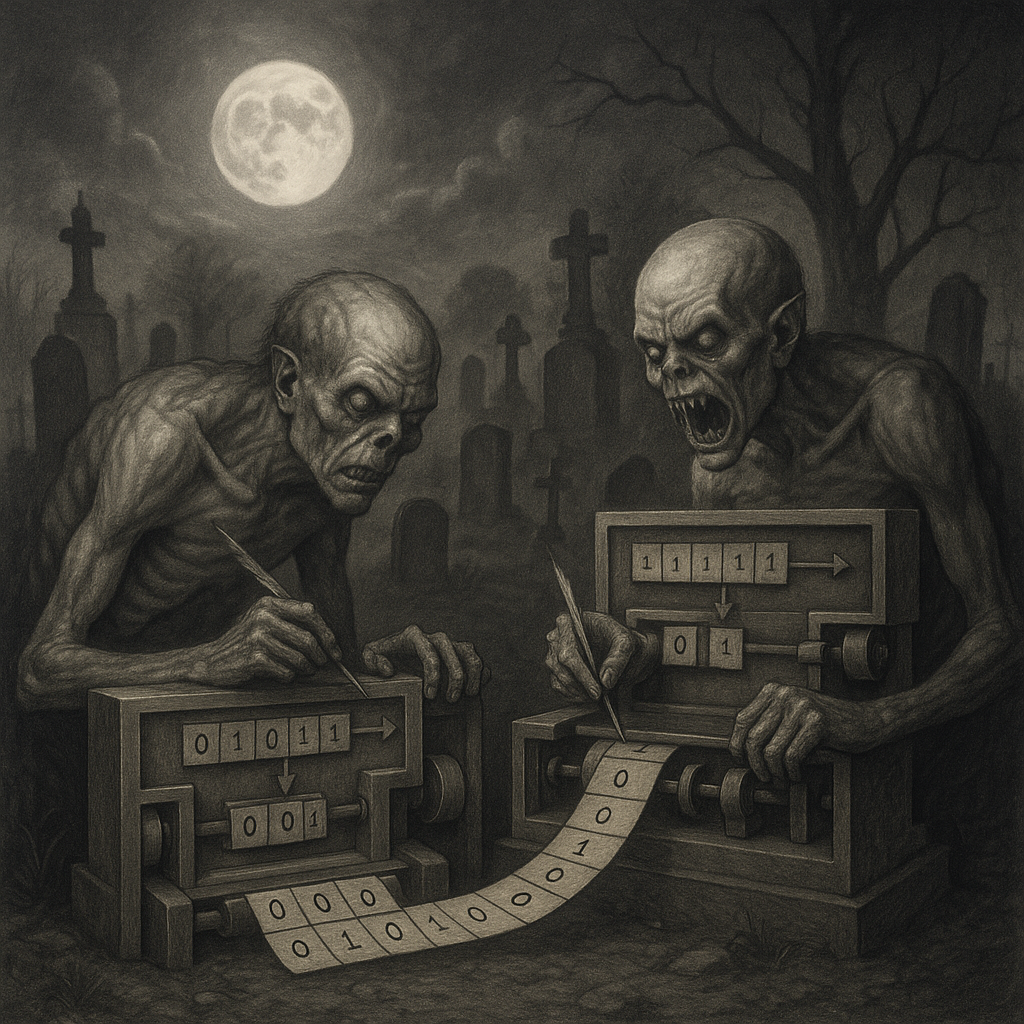
\includegraphics[scale=0.15]{strigoi.png}
\end{center}

Ana și Ecaterina se plictisesc. În cei $400$ de ani de când bântuie \textit{Padurea Codrilor Întunecați}, singura lor distracție sunt rarii călători rătăciți. Așadar, ele s-au apucat de informatică. 

\vspace{1em}

După ce au învățat de concepte precum \textit{Object Oriented Programming} și \textit{Data Oriented Programming}, cele două au inventat paradigma de \textit{Comment Oriented Programming}. Un program se numește \textit{comment-complet} dacă poate evalua orice funcție prin comentarea (ștergerea) unor linii de cod.

Pentru a testa noul concept, cele două vor să creeze un program \textit{comment-complet} care să evalueze polinoame. Își propun să rezolve următorul scenariu:

\begin{enumerate}
    \item Ana alege un număr $N$, pe care îl spune Ecaterinei.
    \item Ecaterina îi spune Anei un program \textit{comment-complet} pentru polinoamele de grad $N$.
    \item Ana alege un polinom $P$ de grad $N$, cu coeficienții numere naturale, pe care îl spune Ecaterinei.
    \item Ecaterina îi spune Anei care linii din programul ei trebuie comentate, pentru ca programul obținut să calculeze $P(X)$.
\end{enumerate}



Instrucțiunile permise în program sunt:
\begin{itemize}
    \item \code{\$VAR1 = \$VAR2 [+-*] \$VAR3} -- Valoarea variabilei \code{\$VAR1} devine suma / diferența / produsul variabilelor \code{\$VAR2} și \code{\$VAR3};
    \item \code{\$VAR1 = \$VAR2 [+-*] A} -- Valoarea variabilei \code{\$VAR1} devine suma / diferența / produsul variabilei \code{\$VAR2} și numărul \textbf{natural} \code{A};
    \item \code{\$VAR1 = A} -- Valoarea variabilei \code{\$VAR1} devine numărul \textbf{natural} \code{A};
\end{itemize}

Variabilele pot avea orice nume format din litere, cifre și underscore (\code{"_"}), și există două variabile speciale:
\begin{itemize}
    \item \code{\$X}: Variabila reprezintă valoarea în care dorim să evaluăm polinomul $P$.
    \item \code{\$Y}: După executarea programului, această variabilă trebuie să fie egală cu $P(\$X)$.
\end{itemize}


\subsection*{Interacțiune}

Întâi citiți gradul $N$ al polinomului.

După aceea, afișați pe o linie $L$, reprezentând numărul de instrucțiuni, urmat de $L$ linii, programul \textit{comment-complet}.

După ce ați afișat programul (\textbf{doar după}), veți putea citi valorile $P_0, P_1, \dots, P_N$, coeficienții polinomului $P$.

După ce ați citit polinomul $P$, afișați $C$, numărul de linii de comentat, urmat de $C$ valori, indicii linilor (indexate de la $0$).

\textbf{Atenție:} Nu uitați să dați flush la \code{stdout} cu \code{cout.flush()} (C++) sau \code{fflush(stdout)} (C).

\subsection*{Constrângeri}

\begin{itemize}
    \item $0 \leq N \leq 10^3$.
    \item $0 \leq P_i \leq 10^9 \ \ \forall 0 \leq i \leq N$  \textbf{(Important)}.
    \item Programul generat poate avea cel mult $2 * 10^5$ operații.
\end{itemize}


\subsection*{Subtask-uri}

\begin{enumerate}
    \item ($20$ de puncte) $N = 1$ și $0 \leq P_i \leq 100 \ \ \forall 0 \leq i \leq N$.
    \item ($20$ de puncte) $0 \leq N \leq 100$ și $0 \leq P_i \leq 100 \ \ \forall 0 \leq i \leq N$.
    \item ($30$ de puncte) $N = 0$.
    \item ($30$ de puncte) Nicio constrângere suplimentară.
\end{enumerate}

% \subsection*{Atașamente}

% Pentru a simplifica testarea soluțiilor, în secțiunea "\textit{Downloads}" a interfeței de concurs puteți descărca un validator pentru soluția voastră.

\subsection*{Exemplu}

\textbf{Notă}: Programul afișat în acest exemplu este \textit{comment-complet} numai pentru polinoame cu coeficienții cel mult $2$.

\begin{tabular}{|@{}p{0.5\textwidth}@{}|@{}p{0.5\textwidth}@{}|}
\hline
\multicolumn{1}{|c|}{\bfseries Input Standard (\textit{cin})} &
\multicolumn{1}{c|}{\bfseries Output Standard (\textit{cout})} \\
\hline
\begin{textQuoteCell}
1








1 2
\end{textQuoteCell} &
\begin{textQuoteCell}

8
$Y0 = 0
$Y0 = 1
$Y0 = 2
$Y1 = 0
$Y1 = 1
$Y1 = 2
$Y1 = $Y1 * $X
$Y = $Y0 + $Y1

4
0 2 3 4
\end{textQuoteCell} \\    
\hline
\begin{textQuoteCell}
1








0 1
\end{textQuoteCell} &
\begin{textQuoteCell}

8
$Y0 = 0
$Y0 = 1
$Y0 = 2
$Y1 = 0
$Y1 = 1
$Y1 = 2
$Y1 = $Y1 * $X
$Y = $Y0 + $Y1

4
1 2 3 5
\end{textQuoteCell} \\    
\hline
\end{tabular}


\subsection*{Explicație Exemplu}

Considerăm primul exemplu.

\subsubsection*{Pas 1}

Ana a ales un polinom de grad $1$. Așadar, îi transmite Ecaterinei numărul $1$.

\subsubsection*{Pas 2}

Ecaterina răspunde cu următorul program:
\begin{center}
\begin{tabular}{c}
\begin{lstlisting}[language=Bash]
$Y0 = 0
$Y0 = 1
$Y0 = 2
$Y1 = 0
$Y1 = 1
$Y1 = 2
$Y1 = $Y1 * $X
$Y = $Y0 + $Y1
\end{lstlisting}
\end{tabular}
\end{center}

\subsection*{Pas 3}

Ana îi spune Ecaterinei că a ales polinomul $P(X) = 1 + 2*X$.

\subsection*{Pas 4}

Ecaterina îi spune Anei că pentru ca programul pe care l-a afișat la pasul 2 să evalueze polinomul P, trebuie comentate liniile $0, 2, 3$ și $4$.

\subsection*{Verificare}

După comentarea liniilor, codul Ecaterinei devine:
\begin{center}
\begin{tabular}{c}
\begin{lstlisting}[language=Bash]
$Y0 = 1
$Y1 = 2
$Y1 = $Y1 * $X
$Y = $Y0 + $Y1
\end{lstlisting}
\end{tabular}
\end{center}

Putem să observăm așadar că $\$Y = 1 + 2 * \$X = P(\$X)$. 

\end{document}